\chapter{Group comparison and summary}

\section{Offered functionalities}

Libraries discussed within this dissertation differ in types and numbers of offered functionalities. The table \ref{fun:sum} summarizes each aspects shown in the previous chapters.

\begin{longtable}{c | c | c | c}
	\centering
	\multirow{2}{*}{\makecell{Funkcjonalność}} & \multicolumn{3}{c}{Biblioteka} \\
	\cline{2-4}
	 &  Shogun & Shark-ML & Dlib \\
	\hline
	\makecell{Odczyt \\ danych} & \makecell{std::vector, \\ wsparcie dla \\ formatu CSV} & \makecell{surowe \\ tablice, \\ wsparcie dla \\ formatu CSV, \\ wsparcie \\ dla HTTP} & \makecell{std::vector, \\ wsparcie dla \\ formatu CSV} \\
	\hline
	{Normalizacja} & min-max & \makecell{przedział \\ jednostkowy, \\ jednostkowa \\ wariancja, \\ zerowa \\ średnia i \\ wybrana \\ wariancja} & standaryzacja \\
	\hline
	\makecell{Redukcja \\ wymiarowości} & \makecell{PCA, Kernel PCA, \\ MDS, IsoMap, \\ ICA, Factor analysis, \\t-SNE} & \makecell{PCA, Liniowa \\ analiza \\ dyskryminacyjna} & \makecell{PCA, Liniowa \\ analiza \\ dyskryminacyjna, \\ Mapowanie \\ Sammona} \\
	\hline
	\makecell{Regularyzacja} & \makecell{L1 i L2 \\ automatyczna} & \makecell{L1 i L2} & L2 \\
	\hline
	\makecell{Regresja \\ liniowa} & Tak & Tak & Tak \\
	\hline
	\makecell{Regresja \\ logistyczna} & Tak & Tak & Nie \\
	\hline
	\makecell{Maszyna \\ wektorów \\ nośnych} & Tak & Tak & Tak \\
	\hline
	\makecell{Algorytm \\ K-najbliższych \\ sąsiadów} & Tak & Tak & Nie \\
	\hline
	\makecell{Algorytm \\ zbiorowy} & \makecell{Wzmacnianie \\ gradientu, \\ losowy las} & \makecell{Losowy \\ las} & Nie \\
	\hline
	\makecell{Sieć \\ neuronowa} & Tak & Tak & Tak \\
	\hline
	\makecell{Jądrowa \\ regresja \\ grzbietowa} & Nie & Nie & Tak \\
	\hline
	\makecell{Błąd \\ średniokwadratowy} & Tak & Tak & Nie \\
	\hline
	\makecell{Średni \\ błąd \\ bezwzględny} & Tak & Tak & Nie \\
	\hline
	\makecell{Błąd typu \\ zero-jeden} & Nie & Tak & Nie \\
	\hline
	\makecell{Błąd \\ dyskretny} & Nie & Tak & Nie \\
	\hline
	\makecell{Entropia \\ krzyżowa} & Nie & Tak & Nie \\
	\hline
	\makecell{Kawałkami \\ liniowa \\ funkcja straty} & Nie & Tak & Nie \\
	\hline
	\makecell{Średnio-\\kwadratowy \\ błąd typu \\ kawałkami \\ liniowej \\ funkcji straty} & Nie & Tak & Nie\\
	\hline
	\makecell{Kawałkami \\ liniowa \\ funkcja straty \\ typu epsilon} & Nie & Tak & Nie\\
	\hline
	\makecell{Średnio-\\kwadratowy \\ błąd kawałkami \\ liniowej funkcji \\ straty typu \\ epsilon} & Nie & Tak & Nie\\
	\hline
	\makecell{Funkcja \\ straty \\ Hubera} & Nie & Tak & Nie\\
	\hline
	\makecell{Funkcja \\ straty \\ Tukeya} & Nie & Tak & Nie\\
	\hline
	\makecell{Logarytmiczna \\ funkcja \\ straty} & Tak & Nie & Nie\\
	\hline
	\makecell{Metryka $R^2$} & Tak & Tak & Nie\\
	\hline
	\makecell{Dokładność} & Tak & Nie & Tak \\
	\hline
	\makecell{Pole pod \\ wykresem \\ ROC} & Tak & Tak & Tak* \\
	\hline
	\makecell{Sprawdzian \\ krzyżowy \\ k-krotny} & Tak & Tak & Tak \\
	\caption{Zbiorcze porównanie funkcjonalności bibliotek.}
	\label{fun:sum}
\end{longtable} 

* - need to calculate the area under ROC curve using data points of the function plot.

By analyzing the data collected in the table \ref{fun:sum} it can be noticed, that the Shogun and Shark-ML libraries are fairly similar with types and number of available machine learning methods, however Shark-ML contains significantly more loss function types which can be used, allowing for more freedom when customizing the training process. The least amount of functionalities is displayed by the Dlib library, which contain only a subset of the algorithms present in the other projects. What is more, it has very limited model quality analysis possibilities, requiring making of own procedures for data processing by the user, such as eg. area under ROC curve calculation procedure.

\section{Comparison of the results from test examples}

In order to test the proficiency of each library, they were used for creating and evaluating linear regression and support vector machine models for the datasets discussed in chapter 3. Each model uses 80\% of the dataset for training, and the remaining 20\% as validation. Table \ref{tab:models} shows group comparison of achieved results. Output of the programs utilizing the libraries was presented on figures \ref{fig:shogun_linear_svm}, \ref{fig:shark_linear_svm} and \ref{fig:dlib_linear_svm}.

\newpage
\begin{longtable}{c | c | c }
	\centering
	\multirow{2}{*}{\makecell{Biblioteka}} & \multicolumn{2}{c}{Metoda uczenia maszynowego} \\
	\cline{2-3}
	& Regresja liniowa & Maszyna wektorów nośnych \\
	\hline
	\makecell{Shogun} & \makecell{Dane treningowe: \\ MSE = 0,903031; $R^2$ = 0,407058 \\ Dane testowe: \\ MSE = 1,26897; $R^2$ = -0.127851} & \makecell{Dane treningowe: \\ AUC ROC: 1 \\ Dane testowe: \\ AUC ROC: 0,5} \\
	\hline
	\makecell{Shark} & \makecell{Dane treningowe: \\ MSE = 0,38728; $R^2$ = 0,745707 \\ Dane testowe: \\ MSE = 0,449118; $R^2$ = 0,60082} & \makecell{Dane treningowe: \\ AUC ROC: 1 \\ Dane testowe: \\ AUC ROC: 0,5} \\
	\hline
	\makecell{Dlib} & \makecell{Dane treningowe: \\ MSE = 3,08953; \\ Dane testowe: \\ MSE = 1,33014; } & \makecell{Dane treningowe: \\ AUC ROC: 1 \\ Dane testowe: \\ AUC ROC: 1} \\
	\caption{Zestawienie uzyskanych wyników poprawności modeli.}
	\label{tab:models}
\end{longtable} 

\begin{figure}[!ht]
	\centering
	\begin{minipage}{0.31\textwidth}
		\centering
		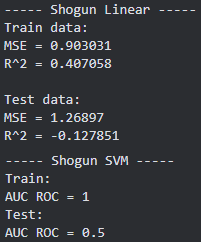
\includegraphics[width=0.8\linewidth]{Rozdzial7/shogun}
		\caption{Wynik działania programu dla biblioteki Shogun}
		\label{fig:shogun_linear_svm}		
	\end{minipage}%
    \hspace{0.02\textwidth}
	\begin{minipage}{0.31\textwidth}
		\centering
		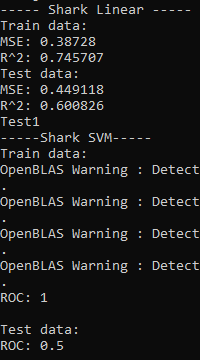
\includegraphics[width=0.7\linewidth]{Rozdzial7/shark}
		\caption{Wynik działania programu dla biblioteki Shark}
		\label{fig:shark_linear_svm}		
	\end{minipage}%
	\hspace{0.02\textwidth}
	\begin{minipage}{0.31\textwidth}
		\centering
		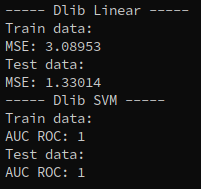
\includegraphics[width=0.8\textwidth]{Rysunki/Rozdzial7/dlib}
		\caption{Wynik działania programu dla biblioteki Dlib}
		\label{fig:dlib_linear_svm}
	\end{minipage}
\end{figure}

By analyzing the above results for linear regression, it can be concluded that the first place was taken by the Shark-ML library, which is characterized by the least values of the mean squared error. On second place is Shogun library. It can be noticed that the $R^2$ calculation mechanism crossed outside the allowed interval for the metric for validation data. It is suspected that it is a result of cumulative floating point representation errors during calculations, pointing that the mechanism of calculating the $R^2$ metric components may be numerically unstable. The last place was taken by Dlib, in case of which the value of mean squared error exceeded 3 units.

Much worse results were acquired for the classification task using the aforementioned libraries. Each of them is characterized by seemingly perfect fit to the training data, and in case of Shark-ML and Shogun libraries, a fit equal to coin flip for the validation data. The Dlib library additionally achieved the area under the ROC curve equal to 1 for the validation data. Above results are considered impossible to achieve, which was proven in chapter 3 section 3.3.1 using dedicated statistical software. Because of that, and analysis of the causes was undertaken.

In order to improve the acquired results and to solve encountered errors it was decided to normalize the predictor values for both datasets into an interval of $\langle0; 1\rangle$ using JMP software, and subsequently to analyze the code which performs the support vector machine training for each of the libraries. First of them was Shark-ML, where manual tuning of gamma and regularization parameters was applied. It turned out that after data normalization, setting gamma parameter to 0.16 and setting regularization to 1 a correct and plausible result was achieved, where the area under the ROC curve is equal to 0.933129 for the validation data. Next the Shogun library was tested. Unfortunately, despite data normalization, the problem of the $R^2$ metric value crossing boundaries for validation data was not solved. However, a successful classification was performed, acquiring the value of the area under the ROC curve equal to 0.638112. It is important to notice, that the normalization process made the achieved regression results worse for the Shogun library, decreasing the $R^2$ metric for training data, and making the value of this metric for validation data stray even further from its correct boundaries. The last of the libraries was Dlib, for which the data normalization significantly improved acquired mean square error values, however the support vector machine still achieved a perfect fit, which can point to the fact, that the mechanism might be implemented incorrectly. Table \ref{tab:models2} summarizes the results achieved after code analysis and data normalization. Output of the programs was presented on figures \ref{fig:shogun_linear_svm2}, \ref{fig:shark_linear_svm2} and \ref{fig:dlib_linear_svm2}.

\begin{longtable}{c | c | c }
	\centering
	\multirow{2}{*}{\makecell{Biblioteka}} & \multicolumn{2}{c}{Metoda uczenia maszynowego} \\
	\cline{2-3}
	& Regresja liniowa & Maszyna wektorów nośnych \\
	\hline
	\makecell{Shogun} & \makecell{Dane treningowe: \\ MSE = 0,0286481; $R^2$ = 0,3127 \\ Dane testowe: \\ MSE = 0.0427863; $R^2$ = -0.389462} & \makecell{Dane treningowe: \\ AUC ROC: 0,789143 \\ Dane testowe: \\ AUC ROC: 0,638112} \\
	\hline
	\makecell{Shark} & \makecell{Dane treningowe: \\ MSE = 0,0105995; $R^2$ = 0,745707 \\ Dane testowe: \\ MSE = 0.0122919; $R^2$ = 0,600826} & \makecell{Dane treningowe: \\ AUC ROC: 0,921643 \\ Dane testowe: \\ AUC ROC: 0,933129} \\
	\hline
	\makecell{Dlib} & \makecell{Dane treningowe: \\ MSE = 0,481402; \\ Dane testowe: \\ MSE = 0,179538; } & \makecell{Dane treningowe: \\ AUC ROC: 1 \\ Dane testowe: \\ AUC ROC: 1} \\
	\caption{Zestawienie uzyskanych wyników poprawności modeli.}
	\label{tab:models2}
\end{longtable} 

To summarize, it was noticed that each of the libraries is especially sensitive to the value ranges of the predictors, and in order to properly use them, in most cases it is needed that the predictors values are contained within the interval of $\langle0; 1\rangle$. It was especially visible in case of the classification dataset, where due to the inverse Arrhenius transformation there was a significant discrepancy between the value range of those predictors, and the intervals of other predictors. Additionally it was noticed, that the mechanism of calculating the $R^2$ metric within the Shogun library and support vector machine in Dlib library likely contain implementation errors, so it is recommended to either not use them, or to have a very limited trust to them. Among the achieved results, the best fit was present in case of Shark-ML library, with Shogun on second place and Dlib on the last place.

\begin{figure}[!ht]
	\centering
	\begin{minipage}{0.31\textwidth}
		\centering
		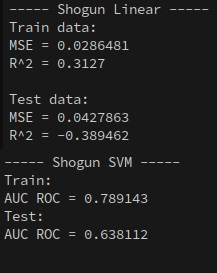
\includegraphics[width=0.8\linewidth]{Rozdzial7/shogun_linear_svm}
		\caption{Wynik działania programu dla biblioteki Shogun}
		\label{fig:shogun_linear_svm2}		
	\end{minipage}%
	\hspace{0.02\textwidth}
	\begin{minipage}{0.31\textwidth}
		\centering
		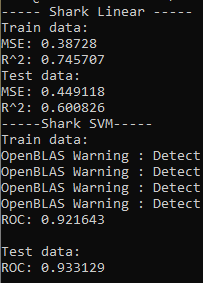
\includegraphics[width=0.7\linewidth]{Rozdzial7/shark_linear_svm}
		\caption{Wynik działania programu dla biblioteki Shark}
		\label{fig:shark_linear_svm2}		
	\end{minipage}%
	\hspace{0.02\textwidth}
	\begin{minipage}{0.31\textwidth}
		\centering
		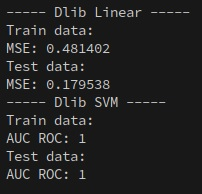
\includegraphics[width=0.8\textwidth]{Rysunki/Rozdzial7/dlib_linear_svm}
		\caption{Wynik działania programu dla biblioteki Dlib}
		\label{fig:dlib_linear_svm2}
	\end{minipage}
\end{figure} 

\section{Sources quality and needed effort}

During working with each of the libraries it was noticed, that the least amount of effort was needed when working with Shark-ML library. It is due to the very user-friendly syntax and precise documentation available on the project's main website, alongside use examples for each of the methods. The library was also effortlessly build and installed in the Ubuntu 22.04 system in the WSL2 environment, allowing to quickly move along with the research.

The second library in the effort metric turned out to be the Dlib toolbox. It has its own project website with all the available classes and functions listed, however the description of each method is very short, and there is a lack of available examples. The syntax can prove challenging to the user, as it is not always obvious and sometimes makes the analysis of the performed operations harder.

The most effort-intensive library was Shogun. During the making of this dissertation, both official repository of the project, and the repository of Ubuntu operation system turned out to be incomplete. It rendered installing the library using the in-built packet manager impossible, aswell as building it due to the not fixed dependencies to moved external repositories. Despite slightly more user-friendly syntax than the Dlib library, previously mentioned issue caused that in order to download the library, it was necessary to install a special packet manager called \textit{nix} which contain an older version of the Shogun project in its own repository. Because of the lack of documentation and the fact, that the generated examples do not use API provided by the library, and instead use it in completely separate, unnatural for the project way, researching the functionalities and the way to implement each of the machine learning tasks had to be based almost solely on the book sources. It significantly impares and prolongs the process of utilizing it into any project.